\section{}
The system shown in the figure is used to accurately measure changes when the pressure 
is increased by $\Delta P$ in the water pipe. When $\Delta h = 70$ mm, what is the change 
in the pipe pressure?

\begin{figure}[h]
    \centering
    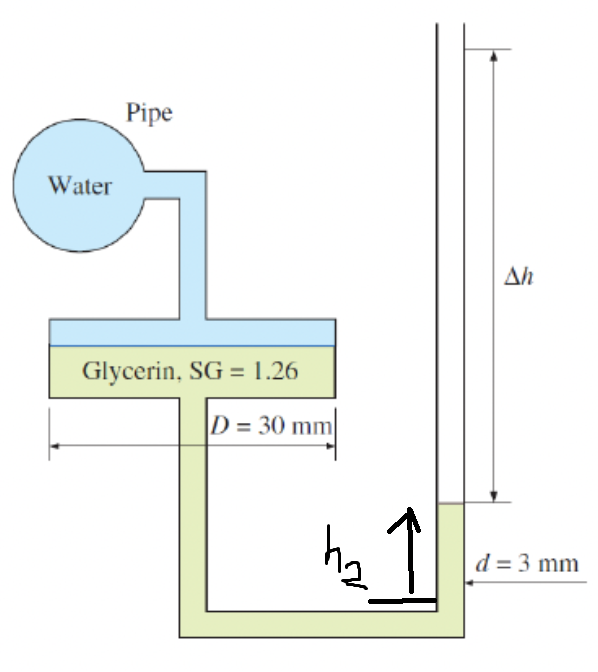
\includegraphics[width=0.3\textwidth]{Questions/Figures/Q3ProblemDiagram.png}
    \caption{Convoluted manometer diagram}
    \label{fig:Q3ProblemDiagram}
\end{figure}

Assumptions:
\begin{itemize}
    \item $x$ is less than $l$
    \item Density is constant
    \item The manometer is open to the atmosphere
\end{itemize}

By conservation of mass, the volume displaced on the right side of the manometer is equal to the volume displaced on the left side of the manometer. 

\begin{align}
    \Delta V_{left} &= \Delta V_{right} \nonumber \\
    \Delta h \left(\frac{\pi}{4} D_{right}^2\right) &= x \left(\frac{\pi}{4} D_{left}^2\right) \nonumber \\
    \implies x &= \Delta h \left(\frac{D_{right}}{D_{left}}\right)^2 \label{eq:Q3x} \nonumber \\
    &= 70 \times \left(\frac{3}{30}\right)^2 \nonumber \\
    &= \qty{0.7}{\milli\meter} \nonumber
\end{align}

In the initial state, the pressure balance going from the water to the air is (look at where the fluid starts and ends; 
downwards displacement is positive, upwards displacement is negative):
\begin{equation}
    P_{w, 1} + \rho_{w} g h_1 + \rho_{g} g (h_2 - h_1) = P_{atm} \label{eq:Q3State1}
\end{equation}

In the final state, the pressure balance is:
\begin{equation}
    P_{w, 2} + \rho_{w} g (h_1 + x) + \rho_{g} g (h_2 - \Delta h - x - h_1) = P_{atm} \label{eq:Q3State2}
\end{equation}

Subtracting (\ref{eq:Q3State1}) from (\ref{eq:Q3State2}) yields:
\begin{equation}
    P_{w, 2} - P_{w, 1} = -\rho_{w} g x + \rho_{g} g (\Delta h + x) \label{eq:Q3DeltaP}
\end{equation}

To find the density of glycerin given SG = 1.26, we can use the following equation:
\begin{equation}
    \rho_{g} = \rho_{H_2O} \times SG = 1000 \times 1.26 = \qty{1260}{\kilogram\per\meter\cubed} \nonumber
\end{equation}

Substituting this into (\ref{eq:Q3DeltaP}) yields:
\begin{equation}
    \Delta P = -1000 \times 9.81 \times \frac{0.7}{1000} + 1260 \times 9.81 \times \frac{70 + 0.7}{1000} = \boxed{\qty{867.0}{\pascal}} \nonumber
\end{equation}